\documentclass[14pt]{beamer}

\mode<presentation> {
\usetheme{Madrid}

% To remove the navigation symbols from the bottom of all slides uncomment next line
\setbeamertemplate{navigation symbols}{} 
\date{}
\title{}
\author{}

%to get rid of footer entirely uncomment next line
\setbeamertemplate{footline}{}
}


\usepackage{geometry}
\usepackage{multirow}
\usepackage{adjustbox}
\usepackage{multicol}
\setlength{\columnsep}{0.1cm}



\usepackage{tikz}
\usetikzlibrary{shapes,backgrounds}

\usepackage{bbding}
\usepackage{rotating}
\usepackage{xcolor}


%\usepackage{tkz-berge} %cool grid
\usepackage{pgfplots} %pics

\usepackage{graphicx} % Allows including images
\usepackage{booktabs} % Allows the use of \toprule, \midrule and \bottomrule in tables
\usepackage{mathtools}

\newcommand {\DS} [1] {${\displaystyle #1}$}
\newcommand {\R}{\mathbb{R}}
\newcommand {\Z}{\mathbb{Z}}
\newcommand {\N}{\mathbb{N}}
\newcommand{\e}{\varepsilon}

\newcommand{\p}{\pause}

% simple environrment for enumerate, easier to read
\setbeamertemplate{enumerate items}[default]

%%%%%%%%%%%%%%%%%%%%%%

% to use colours easily
\definecolor{verde}{rgb}{0, .8, 0} 
\definecolor{rosa}{rgb}{1, 0, 1}  
\definecolor{naranja}{rgb}{1, .5, 0.1} 
\newcommand{\azul}[1]{{\color{blue} #1}}
\newcommand{\rojo}[1]{{\color{red} #1}}
\newcommand{\verde}[1]{{\color{verde} #1}}
\newcommand{\rosa}[1]{{\color{rosa} #1}}
\newcommand{\naranja}[1]{{\color{naranja} #1}}
\newcommand{\violeta}[1]{{\color{violet} #1}}

 
% box in red and blue in math and outside of math
\newcommand{\cajar}[1]{\boxed{\mbox{\rojo{ #1}}}}
\newcommand{\majar}[1]{\boxed{\rojo{ #1}}}
\newcommand{\cajab}[1]{\boxed{\mbox{\azul{ #1}}}}
\newcommand{\majab}[1]{\boxed{\azul{ #1}}}
 
\newcommand{\setsize}[1]{\fontsize{#1}{#1}\selectfont} %allows you to change the font size. The default size of this document is 14. To change the font size of the whole slide, place this at the beginning of the slide. To change the size of only a portion of the text to size 12, you can do the following { \setsize{12} Your text. }.

\setbeamerfont{frametitle}{size=\setsize{15}}
\setbeamerfont{block title}{size=\setsize{14}}

\newcommand{\smallerfont}{\setsize{13}} %place this at the beginning of a slide to set the font size of the entire slide to 13.

%===========================
% Preamble just for this file
%===========================

\newcommand{\arcsec}{\operatorname{arcsec}}

%===================================================
\begin{document}
%===================================================

%-----------------------------
\begin{frame}
\frametitle{Definition of local extremum}

Find local and global extrema of the function with this graph:

\begin{center}
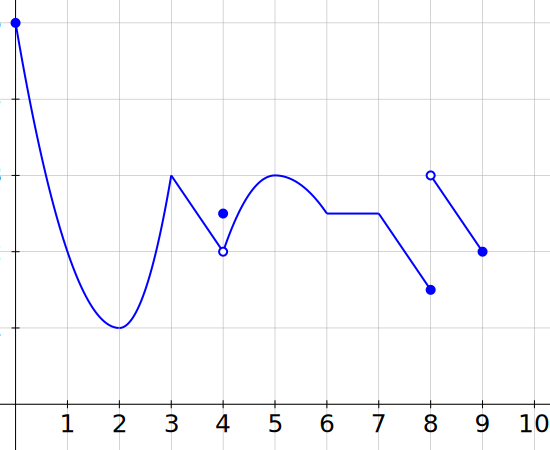
\includegraphics[scale=.42]{G13}
\end{center}

\end{frame}
%-----------------------------
\begin{frame}[t]
\frametitle{Where is the maximum?}

We know the following about the function $h$:
	\begin{itemize}
		\item  The domain of $h$ is \DS{(-4,4)}.
		\item  $h$ is continuous on its domain.
		\item  $h$ is differentiable on its domain, except at $0$.
		\item  $h'(x) = 0 \quad \iff \quad x=-1 \mbox{ or } 1$.
	\end{itemize}
	
\begin{block}{What can you conclude about the maximum of $h$?}
\pause
	\begin{enumerate}
		\item  $h$ has a maximum at $x=-1$, or $1$.
		\item  $h$ has a maximum at $x=-1,0,$ or $1$.
		\item  $h$ has a maximum at $x=-4, -1,0, 1,$ or $4$.
		\item None of the above.	
	\end{enumerate}
\end{block}	


\end{frame}
%-----------------------------
\begin{frame}[t]
\frametitle{What can you conclude?}

We know the following about the function $f$.
	\begin{itemize}	
		\item  $f$ has domain $\R$.
		\item  $f$ is continuous
		\item  $f(0)=0$
		\item  For every $x \in \R$, $f(x) \geq x$.
 	\end{itemize}
\begin{block}{}
What can you conclude about $f'(0)$?  Prove it.
\end{block}

\vfill

\emph{Hint:}  Sketch the graph of $f$.   Looking at the graph, make a conjecture. \\
To prove it, imitate the proof of the Local EVT from Video 5.3.



\end{frame}

%-----------------------------
\begin{frame}[t]
\frametitle{Fractional exponents}

Let
	\DS{
		g(x) = x^{2/3} (x-1)^3.
	}
	
\

Find local and global extrema of $g$ on \DS{[-1,2]}.

\end{frame}
%-----------------------------
\begin{frame}[t]
\frametitle{Trig extrema}

Let
	\DS{
		f(x) = \frac{\sin x}{3 + \cos x}.
	}

\
	
Find the maximum and minimum of $f$.

\end{frame}
%-----------------------------
\begin{frame}[t]
\frametitle{How many zeroes?}

Let
	$$
		f(x) = e^x - \sin x + x^2 + 10x
	$$
	
How many zeroes does $f$ have?
	
\end{frame}
%-----------------------------
\begin{frame}[t]
\frametitle{Zeroes of the derivative}

Sketch the graph of a function $f$ that is differentiable on $\R$ and such that

\

	\begin{enumerate}
		\item $f$ has exactly 3 zeroes and $f'$ has exactly 2 zeroes.
		\item $f$ has exactly 3 zeroes and $f'$ has exactly 3 zeroes.
		\item  $f$ has exactly 3 zeroes and $f'$ has exactly 1 zero.
		\item  $f$ has exactly 3 zeroes and $f'$ has infinitely many zeroes.
	\end{enumerate}


\end{frame}
%-----------------------------
\begin{frame}[t]
\frametitle{Zeroes of a polynomial}

You probably learned in high school that a polynomial of degree $n$ has at most $n$ real zeroes.  Now you can prove it!

\

\emph{Hint:}  Use induction.  If you are having trouble, try the case $n=3$ first.


\end{frame}
%-----------------------------
\begin{frame}[t]
\frametitle{The second Theorem of Rolle}

Complete statement for this theorem and prove it.

\vfill

\begin{block}{Rolle's Theorem 2}
Let $a<b$.  Let $f$ be a function defined on $[a,b]$. \\
IF
	\begin{itemize}
		\item  (Some conditions on continuity and derivatives)
		\item  \DS{f(a) = f'(a) =0}
		\item  \DS{f(b)=0}
	\end{itemize}
THEN \DS{\exists c \in (a,b)} such that \DS{f''(c)=0}.
\end{block}

\vfill

\emph{Hint:}  Apply the 1st Rolle's Theorem to $f$, then do something else.

\end{frame}
%-----------------------------
\begin{frame}[t]
\frametitle{The $N$-th Theorem of Rolle}

Complete the statement for this theorem and prove it.

\

\begin{block}{Rolle's Theorem $N$}
Let $N$ be a positive integer. \\
Let $a<b$.  Let $f$ be a function defined on $[a,b]$. \\
IF
	\begin{itemize}
		\item  (Some conditions on continuity and derivatives)
		\item  (Some conditions at $a$)
		\item  \DS{f(b)=0}
	\end{itemize}
THEN \DS{\exists c \in (a,b)} such that \DS{f^{(N)}(c)=0}.
\end{block}


\end{frame}

%-----------------------------

\begin{frame}[t]
\smallerfont
\frametitle{A new theorem}

We want to prove this theorem:
\begin{block}{\smallerfont Theorem 1}
Let $f$ be a differentiable function on an open interval $I$. \\
IF
	\DS{\forall x \in I, f'(x) \neq 0} \\
THEN
	$f$ is one-to-one on $I$.
\end{block}

\vfill \pause

\begin{enumerate}
	\item Transform  \quad \DS{[P \implies Q]} \quad into \quad \DS{ [(\mbox{not } Q) \implies (\mbox{not } P)]}. \\
		You get an equivalent Theorem (call it ``Theorem 2").  \\
		We are going to prove Theorem 2 instead.
	\item  Write the definition of ``$f$ is not one-to-one on $I$".  You will need it.
	\item  Recall the statement of Rolle's Theorem.  You will need it.
	\item  Do some rough work if needed.
	\item  Write a complete proof for Theorem 2.
\end{enumerate}

\end{frame}

%-----------------------------
\begin{frame}[t]
\frametitle{A variant}

Complete this variation on Theorem 2. \\ 
Use the weakest conditions you can to make it true.  

\


\begin{block}{Theorem 3}
Let $a<b$.  Let $f$ be a function defined on $[a,b]$. \\
IF
	\begin{itemize}
		\item (Some conditions on continuity and differentiability)
		\item  $f$ is not one-to-one on $[a,b]$
	\end{itemize}
THEN 
		  \DS{\exists c \in (a,b)} such that $f'(c)=0$.
\end{block}


\end{frame}

%-----------------------------
\begin{frame}
\frametitle{Why the three hypotheses are necessary}

You have proven

\begin{block}{Theorem 3}
Let $a<b$.  Let $f$ be a function defined on $[a,b]$. \\
IF
	\begin{enumerate}
		\item $f$ is continuous on $[a,b]$
		\item $f$ is differentiable on $(a,b)$
		\item  $f$ is not one-to-one on $[a,b]$
	\end{enumerate}
THEN 
		  \DS{\exists c \in (a,b)} such that $f'(c)=0$.
\end{block}


\vfill

Give three examples to justify that each of the three hypotheses are necessary for the theorem to be true.
(Graphs of the examples are enough).


\end{frame}
%-----------------------------
\begin{frame}[t]
\frametitle{MVT -- True or False?}

\begin{block}{True or False}
Consider  $f(x) = |x|$ on the interval
 $[-\frac{1}{2}, 2]$.  
 
 There exists $c$ in $(-\frac{1}{2},2)$ such that
\[f'(c) = \frac{f(2) - f(-\frac{1}{2})}{2-(-\frac{1}{2})}\]
\end{block}
%This is a quick warm up question to make sure that students watched the video and understand that we need to check that all the hypotheses are satisfied before using the theorem.

\end{frame}

%-----------------------------
\begin{frame}[t]
\smallerfont
\frametitle{Car race - 1}

A driver competes in a race.

\

Use MVT to prove that at some point during the race the instantaneous velocity of the driver is exactly equal to the average velocity of the driver during the race.


\end{frame}

%-----------------------------
\begin{frame}[t]
\smallerfont
\frametitle{Car race - 2}

Two drivers start a race at the same moment and finish in a tie.

\

Can you conclude that there was a time in the race (not counting the starting time) when the two drivers had exactly the same speed?

\end{frame}
%-----------------------------
\begin{frame}[t]
\smallerfont
\frametitle{Car race - Is this proof correct?}

\begin{block}{\smallerfont Claim}
IF two drivers start a race at the same moment and finish in a tie, THEN at some point in the race (not counting the starting time) they had exactly the same speed.
\end{block}

{\bf Proof?}
	\begin{itemize}
		\item Let $f(t)$ and $g(t)$ be the positions of the two cars at time $t$.
		\item Assume the race happens in the interval $[t_1,t_2]$.   By hypothesis:
			$$ f(t_1) = g(t_1), \quad \quad f(t_2) = g(t_2). $$
		\item Using MVT, there exists $c \in (t_1, t_2)$ such that
			$$
				f'(c) = \frac{f(t_2) - f(t_1)}{t_2 - t_1}, \quad g'(c) = \frac{g(t_2) - g(t_1)}{t_2 - t_1}.
			$$	
		\item Then $f'(c) = g'(c)$. \hfill $\square$
	\end{itemize}

\end{frame}

%-----------------------------
\begin{frame}[t]
\smallerfont
\frametitle{Car race - resolution}

Two drivers start a race at the same moment and finish in a tie.

\

Prove that at some point during the race (not counting the starting time) the two drivers had exactly the same speed. 

\end{frame}

%-----------------------------
\begin{frame}[t]
\smallerfont
\frametitle{Speeding ticket!}

On a toll road Barney takes a time stamped toll-card from the starting booth and drives directly to the end of the toll section.  \\
\vspace{.2cm}

After paying the required toll, Barney is surprised to receive a speeding ticket along with the toll receipt. \\
\vspace{.2cm}

Which of the following are true?
\vspace{.2cm}
\begin{enumerate}
\item The booth attendant does not have enough information to prove that Barney was speeding.
\item The booth attendant can prove that Barney was speeding during his trip.
\item Barney's ticket is for a lower speed than his actual maximum speed.
\end{enumerate}

\end{frame}
%-----------------------------
\begin{frame}[t]
\frametitle{Proving difficult identities}


\begin{block}{}
Prove that, for every $x \geq 0$,
	$$   2 \arctan \sqrt{x} - \arcsin \frac{x-1}{x+1} =  \frac{\pi}{2}$$
\end{block}


\emph{Hint:} Derivatives. 


	
\end{frame}
%------------------------------------
\begin{frame}[t]
\setsize{12}
\frametitle{Critique this ``proof"}
\begin{itemize}
	\item  \DS{ \phantom{\rojo{\frac{d}{dx}}} \left[  2 \arctan \sqrt{x} -  \arcsin \frac{x-1}{x+1} \right] =  \phantom{\rojo{\frac{d}{dx}}} \left[ \frac{\pi}{2} \right] }
	\item  \DS{ \rojo{\frac{d}{dx}} \left[  2 \arctan \sqrt{x} -  \arcsin \frac{x-1}{x+1} \right] =  \rojo{\frac{d}{dx}} \left[ \frac{\pi}{2} \right] }
	\item  \DS{\frac{2}{1+ \left( \sqrt{x} \right)^2} \cdot \frac{1}{2\sqrt{x}}  \; - \;  \frac{1}{\sqrt{1- \left( \frac{x-1}{x+1} \right)^2}} \cdot \frac{(x+1) - (x-1)}{(x+1)^2} \; = \; 0}
	\item  \DS{\frac{1}{(1+ x)\sqrt{x} }   \; - \;  \frac{1}{  \sqrt{\frac{4x}{(x+1)^2} }} \cdot \frac{2}{(x+1)^2} \; = \; 0}
	\item \DS{0 = 0}
		\item  So \DS{  2 \arctan \sqrt{x} - \arcsin \frac{x-1}{x+1} } is constant.
		\item Evaluate at $x=0$ to find the value of the constant.
		\item \DS{2 \arctan 0 \; - \; \arcsin (-1) \; = \; 0 - \left( - \pi/2 \right) \; = \; \pi/2 }
		\item Therefore, \; \DS{2 \arctan \sqrt{x} - \arcsin \frac{x-1}{x+1} \; = \;  \frac{\pi}{2}}
\end{itemize}



\end{frame}
%-----------------------------
\begin{frame}[t]
\frametitle{Warm up}

\begin{enumerate}

	\item Let $f$ be a function defined on an interval $I$.
	
	Write the definition of ``$f$ is increasing on $I$".
	
	\
	
	\item Write the statement of the Mean Value Theorem.
\end{enumerate}
\end{frame}
%-----------------------------

\begin{frame}[t]
\frametitle{Positive derivative implies increasing}

Use the MVT to prove

\begin{block}{Theorem}
Let $a < b$.  Let $f$ be a differentiable function on $(a,b)$. 
\begin{itemize}
	\item  IF $\forall x \in (a,b), f'(x) >0$,
	\item  THEN $f$ is increasing on $(a,b)$.
\end{itemize}
\end{block}

\pause

\begin{enumerate}
	\item  Recall the definition of what you are trying to prove.
	\item  {\bf From that definition, figure out the structure of the proof.}
	\item  If you have used a theorem, did you verify the hypotheses?
	\item  Are there words in your proof, or just equations?
\end{enumerate}

\end{frame}

%-----------------------------
\begin{frame}[t]
\frametitle{What is wrong with this proof?}

\begin{block}{Theorem}
Let $a < b$.  Let $f$ be a differentiable function on $(a,b)$. 
\begin{itemize}
	\item  IF $\forall x \in (a,b), f'(x) >0$,
	\item  THEN $f$ is increasing on $(a,b)$.
\end{itemize}
\end{block}


\begin{proof}
\begin{itemize}
	\item  From the MVT,
		\DS{
			f'(c) = \frac{f(b) - f(a)}{b-a}
		}
	\item  We know \DS{b-a>0} and  \DS{f'(c)>0}
	\item  Therefore \DS{f(b) - f(a)>0}. \quad  Thus \DS{f(b) > f(a)}.
	\item $f$ is increasing.
\end{itemize}
\end{proof}

\end{frame}
%-----------------------------
\begin{frame}[t]
\frametitle{Your first integration}


  Find all functions $f$ such that, for all \DS{x \in \R}:
		\DS{f''(x) = x + \sin x}.
	
	
\end{frame}

%-----------------------------

\begin{frame}
\frametitle{Intervals of monotonicity}

Let
	\DS{
		g(x) = x^3(x^2-4)^{1/3}.
	}

\
	
	Find out on which intervals this function is increasing or decreasing.
	
	Using that information, sketch its graph.
	
\

	To save time, here is the first derivative:
	$$
		g'(x) = \frac{x^2(11x^2-36)}{3(x^2-4)^{2/3}}
	$$	


\end{frame}

%-----------------------------
\begin{frame}[t]
\smallerfont
\frametitle{True or False -- Monotonicity and local extrema}

Let $I$ be an interval.  Let $f$ be a function defined on $I$.  Let $c \in I$.  
 Which implications are true?

\
\begin{enumerate}
	\item	 IF \rojo{$f$ is increasing on $I$}, \quad  THEN \azul{$\forall x \in I$, $f'(x) >0$}.
	\item	 IF \azul{$\forall x \in I$, $f'(x) >0$}, \quad THEN \rojo{$f$ is increasing on $I$}.
	
	\
	\item  IF \rosa{$f$ has a local extremum at $c$}, \quad THEN \naranja{$f'(c)=0$}.
	\item IF \naranja{$f'(c)=0$}, \quad THEN \rosa{$f$ has a local extremum at $c$}.
	
	\
	\item  IF \rosa{$f$ has local extremum at $c$}, \; THEN \verde{$f$ has an extremum at $c$}
	\item  IF \verde{$f$ has an extremum at $c$}, \; THEN \rosa{$f$ has local extremum at $c$}
\end{enumerate}

\end{frame}

%-----------------------------
\begin{frame}[t]
\frametitle{Inequalities}


Prove that, for every $x \in \R$
	$$
		e^x \geq 1 + x
	$$	
	
\

\emph{Hint:}  Where is the function \DS{f(x) =e^x - 1-x} increasing or decreasing?  What is its minimum?
	
\end{frame}

%-----------------------------
\begin{frame}[t]
\frametitle{Backwards graphing}

Below is the graph of a polynomial $P$.  Notice that it is not at scale.   The coordinates in the graph are $a=24$, $b=25$, and $c=1$.  Find the equation of $P$.

	\begin{center}
	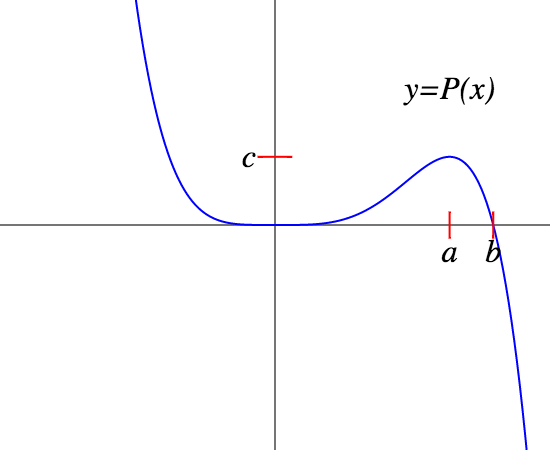
\includegraphics[scale=.38]{G18}
	\end{center}

\end{frame}

%-----------------------------
\begin{frame}[t]
\frametitle{A sneaky function}

Construct a function $f$ satisfying all the following properties:

\

	\begin{itemize}
		\item  Domain \DS{f = \R}
		\item $f$ is continuous
		\item $f'(0)=0$
		\item $f$ does not have a local extremum at $0$.
		\item  There isn't an interval centered at $0$ on which $f$ is increasing.
		\item  There isn't an interval centered at $0$ on which $f$ is decreasing.
	\end{itemize}


\end{frame}

%------------------------------
%-----------------------------
\end{document}
%-----------------------------
%-----------------------------









